\documentclass[conference]{IEEEtran}
\IEEEoverridecommandlockouts

\usepackage[utf8]{inputenc}
\usepackage[T1]{fontenc}
\usepackage{cite}
\usepackage{amsmath,amssymb,amsfonts}
\usepackage{graphicx}
\usepackage{textcomp}
\usepackage{xcolor}
\usepackage{colortbl}
\usepackage{booktabs}
\usepackage{tabularx}
\usepackage{xurl}
\usepackage[hidelinks]{hyperref}
\usepackage{lipsum}

\newcommand{\tbd}[1]{\textcolor{red}{[#1]}}

\begin{document}

\title{Is This Code Mine? Students' Sense of Ownership\\When AI Agents Write Both the Specification and the Code}

\author{\IEEEauthorblockN{Gustavo Pinto}
\IEEEauthorblockA{\textit{Federal University of Pará (UFPA)}\\
Belém, Brazil \\
gpinto@ufpa.br}
\and
\IEEEauthorblockN{Enne Rebeca Silva de Freitas}
\IEEEauthorblockA{\textit{Federal University of Pará (UFPA)}\\
Belém, Brazil \\
enne.freitas@icen.ufpa.br}
\and
\IEEEauthorblockN{Danilo Monteiro Ribeiro}
\IEEEauthorblockA{\textit{CESAR School}\\
Recife, Brazil \\
dmr@cesar.school}
}

\maketitle

\begin{abstract}
Software engineering courses are starting to ask students to build entire systems with AI coding agents, but little is known about what students actually do with them and whether they still own what they deliver. This matters because, if the agent writes both the code and the decisions behind it, the artifacts we grade no longer show what students learned, and we may graduate engineers who ship systems they cannot explain or maintain. In an assignment in which 18 pairs of students built applications with agents under Spec-Driven Development, the agents wrote 69\% of the specifications that were meant to keep the students in control, students credited themselves with half of the ideas but only a fifth of the code, most could neither explain nor modify that code, and the three teams that met the 100,000-line target did so with generated code the application never uses, in one case proposed by the agent itself. Teaching with agents therefore requires assessing what students specify, review, and can explain, rather than what they ship, and enforcing the engineering process with tools rather than trusting it to students or agents.
\end{abstract}

\begin{IEEEkeywords}
AI coding agents, spec-driven development, software engineering education, psychological ownership, mining software repositories
\end{IEEEkeywords}

\section{Introduction}

Today's students will graduate into a profession in which AI coding agents read a code base, plan a change, edit dozens of files, run the tests, and commit the result~\cite{li2026aidev}. Agentic tools are already listed in the syllabi of software engineering courses~\cite{geng2026mapping}, and instructors are rethinking assignments, assessment, and learning goals for a world in which generating code is cheap~\cite{prather2023,denny2024,lau2023ban}. A pair of students can now produce in a few days a volume of code that once required a team and a semester. What they learn by doing so, and what they lose, is an open question for software engineering education.

Most of what we know about students and AI, however, comes from introductory programming, where tasks are small, the solution fits on a screen, and the main concern is whether the tool helps or hinders learning to code~\cite{kazemitabaar2023}. Much less is known about what happens at the other end of the curriculum, when students are asked to use agents on purpose, at a scale they could never reach by hand. At this scale, the question is no longer whether the student wrote the code, but whether the student is still its owner: whether they made the decisions it embodies, know where things are, and feel responsible for its defects. Studies on AI-assisted writing suggest that this feeling may not survive: people do not perceive ownership of AI-generated text, yet still present themselves as its authors~\cite{draxler2024}. If the same happens with code, we may be training engineers who ship systems they do not feel are theirs, and do not know how to maintain.

Spec-Driven Development (SDD) is one of the answers practitioners have proposed to keep humans in control of agents: before asking for code, the developer writes a specification with verifiable acceptance criteria, then a plan, then a list of tasks, and the agent implements one task at a time against the specification~\cite{delimarsky2025speckit,kiro2026specs,piskala2026sdd}. In SDD, the specification is the artifact the human owns, and the code is its consequence. Whether students actually work this way under deadline pressure, and whether owning the specification translates into owning the code, are open questions.

In this paper, we study these questions in a realistic and deliberately extreme setting. In the first assignment of an elective course on AI-assisted software development at the Federal University of Pará, Brazil, 18 pairs of students had to deliver a published application with at least 100,000 lines of code, built with AI coding agents under SDD. Every specification had to be dated and committed before the code it describes, every commit had to declare the agent that produced it and the specification it implements, and every prompt, including the failed ones, had to be recorded in the repository. This setup gives us an unusually complete trace of how the code was produced, which we combine with a survey of the students' perceived ownership. We answer six research questions:

\begin{itemize}
\item[\textbf{RQ1}] \emph{What do students build when asked to deliver 100,000 lines of code with AI coding agents?} We characterize the 18 applications in terms of domain, size, history, and agents used.
\item[\textbf{RQ2}] \emph{To what extent do students follow Spec-Driven Development when working with agents?} We check each repository against the rules of the assignment, such as publishing the application, writing the specification first, and recording every session.
\item[\textbf{RQ3}] \emph{How do students specify software for AI coding agents?} SDD assigns the specification to the human and the code to the agent. We analyze the 277 specifications delivered to find out who wrote them, whether they have the structure the method requires, and whether they actually govern the code.
\item[\textbf{RQ4}] \emph{How much ownership do students perceive over the code, the specification, and the application they delivered?} We survey the students on their perceived ownership, their knowledge of the code, and the share of the ideas and of the code they attribute to themselves and to the agent.
\item[\textbf{RQ5}] \emph{How does perceived ownership relate to the footprint of the agent in the repository?} We relate the answers of each student to the data mined from their repository, including whether their specifications were written by the agent.
\item[\textbf{RQ6}] \emph{How do students game the requirements of the assignment, and what role do AI agents play?} We search the repositories for generated code that inflates the line count and for rewritten history that forges the process record, and trace each case to the commits and sessions that produced it, to understand what the students did and how the agents took part.
\end{itemize}

We found that students built applications in domains such as booking, management, education, finance, and games, but only three of them reached 100,000 lines, and two of these did so mostly with generated code that the application never uses (RQ1). Students followed the conventions of the assignment unevenly: most published the application and wrote dated specifications, but three teams recorded no session at all (RQ2). Most strikingly, the agent wrote not only the code but also most of the specifications: 69\% of them were committed by an agent, and only 1\% were declared as handwritten. Specifications largely had the required structure, but one in four entered the repository in the same commit as the code it describes, few were revised after implementation started, and only 39\% of the added lines can be traced to a specification (RQ3). Students see the ideas as theirs and the code as the agent's: they attribute to themselves a median of 50\% of the ideas but 20\% of the code, only 27\% feel the code is truly theirs, and most could neither explain nor modify it without the agent, even though half feel responsible for its defects (RQ4). Ownership is unrelated to the footprint of the agent in the repository, but related to how much of the generated code students read and, within a pair, to who drove the agent (RQ5). Finally, the size target was gamed: in the three projects that reached it, generated code that the application never uses accounts for 97\%, 99.5\%, and 29\% of the count, in two cases introduced by commits that state the goal of reaching the target, and one team rewrote its history to insert backdated specifications. Agents were involved in every case, but in different roles: in the one case with a recorded session, the agent proposed the generator when the student asked how to reach the target, and in another, an agent warned against inflating the count, to no effect (RQ6).

This paper makes the following contributions:
\begin{itemize}
\item A description of an assignment that asks students to build, with AI coding agents, a system larger than any they could write by hand, with rules that make the use of the agent traceable;
\item An empirical characterization of 18 applications, with 1.4 million lines of code and 1,051 commits, and of how closely students followed SDD;
\item An analysis of how students gamed the requirements of the assignment, of the role AI agents played, and of what made the gaming visible;
\item An analysis of 277 specifications written for AI coding agents, showing that the agent wrote most of the artifact that SDD assigns to the human, and that specifications only partially govern the code;
\item The first study, to the best of our knowledge, of students' perceived ownership of code written with AI coding agents, combining a survey with the mined history of their repositories;
\item \textcolor{red}{An artifact folder with the questionnaire, the anonymized responses, the list of repositories, and the scripts and code used in the analyses (Section~\ref{sec:data}).}
\end{itemize}

\section{Methodology}

\subsection{The Assignment}

The first assignment of the course \emph{AI-Assisted Software Development} (Federal University of Pará, 2026)\footnote{\url{https://gustavopinto.org/teaching/dsai/2026}} was done in pairs, as part of the course. It asked each pair of students to choose and build a non-trivial application with an AI coding agent, following the \emph{spec, plan, tasks} workflow of Spec-Driven Development (SDD) presented in class. Suggested domains included food ordering, ride sharing with trip cost splitting, and place reviews. These were only suggestions: students were free to choose what to build, as well as the stack and the AI tools, as long as they followed the requirements and conventions described below. The assignment was released on September 29, 2026, and students had one week to implement the application. It was the only practical assignment of the term, and the implementation accounted for 30\% of the final grade.

The assignment had four requirements:
\begin{itemize}
\item \textbf{Published.} The application had to open with a single click at a public URL on the day of the presentation.
\item \textbf{100,000 lines.} At least 100,000 lines of code, counted with \texttt{cloc}. Dependencies, lock files, build artifacts, and data did not count.
\item \textbf{SDD.} One dated specification for each part of the system, in a \texttt{SPEC/} folder, written before the code it describes.
\item \textbf{Complete record.} Every prompt, from the first to the last, with the tool and the model used. An application without its prompts would not be graded.
\end{itemize}

\subsection{Repository Conventions}

Each pair created a new public GitHub repository, separate from their course journal, suggested to be named \texttt{dsai-ap1-<app-name>}. Both members had to commit with their own accounts, since the commit author identifies who drove each session, and uploads through the GitHub web interface were not allowed. The repository followed a fixed layout: a \texttt{README.md} with the URL, the pair, the stack, how to run, the tools and models, and the \texttt{cloc} output; a \texttt{SPEC/} folder; free-form \texttt{src/} and \texttt{tests/} folders; and a \texttt{prompts/sessoes/} (\emph{sessions}) folder with the raw session exports. \texttt{PLAN.md}, \texttt{TASKS.md}, and \texttt{AGENTS.md} were optional.

\emph{Specifications.} Each part of the system had its own file, named \texttt{YYYY-MM-DD-<part>.md}, committed before the code it describes, so that the git history shows the order. Small adjustments were edited in place; a change of direction required a new dated file stating which specification it replaces. Each specification describes what is built and why, lists verifiable acceptance criteria, and states what is out of scope. Acceptance criteria are what the agent uses to know when to stop and what the students use to review its output.

\emph{Prompts.} Every prompt counted, including failed and redone ones, one-word prompts such as ``continue'', and prompts issued in other tools, such as a browser chat used to draft a specification. Prompts had to be kept as written, never rewritten afterwards. At the end of each session, the raw export of the tool went into \texttt{prompts/sessoes/}, named \texttt{YYYY-MM-DD-HHMM-<tool>.<ext>}: the session \texttt{.jsonl} for Claude Code, the files under \texttt{\textasciitilde/.codex/sessions/} for Codex CLI, and the conversation export (or a full copy in Markdown) for other tools. Files above 50\,MB were compressed with \texttt{gzip}, and exports had to be checked for secrets before each commit.

\emph{Commits.} Commits had to be small and frequent, at least one per part of the system, and declare their origin in two trailers: \texttt{Agent:} (e.g., \texttt{claude-code/claude-sonnet-5-5}, \texttt{none} for handwritten code, or \texttt{+~manual} for generated and hand-edited code) and \texttt{Spec:}, pointing to the specification the commit implements. History could not be rewritten: no squash, no rebase of pushed commits, and no force push.

\emph{Line count.} Lines were counted only over versioned files, excluding documentation and data:
\begin{center}
\footnotesize
\begin{tabular}{l}
\texttt{cloc . --vcs=git} \\
\texttt{\ \ --exclude-dir=node\_modules,vendor,dist,build,prompts} \\
\texttt{\ \ --exclude-lang=Markdown,JSON,YAML,CSV,Text,SVG} \\
\texttt{\ \ --not-match-f='(lock|\textbackslash.min\textbackslash.)'}
\end{tabular}
\end{center}
The output went into the \texttt{README.md}, with test lines reported separately.

\emph{Presentation.} Without slides, each pair opened the URL live and walked through the main flow, summarized the specification and what was left out, discussed three prompts (the one that worked best, the one that worked worst, and the one that changed the course of the project), and reported the numbers: lines, specifications, prompts, sessions, and hours.

\subsection{Data Collection and Analysis}

On October 7, 2026, we cloned the full history of the 18 repositories submitted. For each repository, we measured source lines with \texttt{cloc} 1.98 using the official command above (Table~\ref{tab:adherence}). We read the \texttt{README.md} to identify the production URL, the tools, and a short description of the application, and we mined the git history to count commits, commits produced by an agent, and commit trailers.

We then checked each repository against the requirements of the assignment:
\begin{itemize}
\item \textbf{URL:} a public production URL is listed in the \texttt{README.md}.
\item \textbf{Specs:} number of Markdown files in \texttt{SPEC/}, and how many follow the dated naming convention.
\item \textbf{Spec first:} among commits whose \texttt{Spec:} trailer points to a file in \texttt{SPEC/}, the share in which that file had been added in an earlier commit.
\item \textbf{Sessions:} number of files in \texttt{prompts/sessoes/}.
\item \textbf{Trailers:} share of commits carrying both \texttt{Agent:} and \texttt{Spec:}.
\item \textbf{Authors:} number of distinct human commit authors (at least two expected).
\item \textbf{SLOC:} line count with the official command (at least 100,000 expected).
\item \textbf{cloc in README:} the \texttt{cloc} output is reported in the \texttt{README.md}.
\item \textbf{Secrets:} versioned files matching common API key patterns (e.g., \texttt{sk-}, \texttt{AKIA}, \texttt{AIza}, \texttt{ghp\_}, private key headers).
\end{itemize}
All checks were automated and are approximate: they rely on file names, trailer formats, and regular expressions, and were not manually validated.

\subsection{Specification Analysis}

To understand how students specified software for the agents, we analyzed every Markdown file under \texttt{SPEC/} in the last commit of each repository, along three dimensions. One team used OpenSpec, another SDD tool, which keeps one specification per capability under \nolinkurl{openspec/changes/<change>/specs/<capability>/spec.md}; we included these files as well.

\emph{Authorship.} For each specification, we identified the commit that added it and classified it as written by an agent when the commit carries an \texttt{Agent:} trailer naming a tool, a \texttt{Co-Authored-By} trailer naming an agent, or an agent as its author; as written by a human when the trailer is \texttt{Agent: none}; and as undeclared otherwise.

\emph{Structure.} The assignment required each specification to state what is built and why, to list verifiable acceptance criteria, and to state what is out of scope. We checked whether each specification has a section for each of these elements, identified by its heading (e.g., ``What and why'', ``Acceptance criteria'', ``Out of scope'', in Portuguese in the original), and counted the acceptance criteria as the list items or table rows under that section, or, in OpenSpec specifications, as the \emph{WHEN}/\emph{THEN} scenarios. We also experimented with lexical indicators of ambiguity (e.g., \emph{fast}, \emph{intuitive}, \emph{properly}) and of verifiability (e.g., numbers, literals, routes), but discarded them after a manual inspection of a sample revealed many false positives, such as ``professional'', which is an entity in a booking system.

\emph{Traceability.} We linked commits to specifications through the \texttt{Spec:} trailer, either by file name or, when students named the part of the system instead of the file (e.g., \texttt{Spec: triagem}, ``triage''), by matching its words with the file name. For each specification, we computed whether at least one commit implements it, whether it was added in the same commit as code, which means it was not written before the code it describes, and whether it was edited after the first commit that implements it, which indicates a specification that evolved with the code. For each repository, we computed the share of added lines, outside \texttt{SPEC/} and \texttt{prompts/}, that come from commits pointing to an existing specification.

As with the adherence checks, these analyses are automated and approximate, and depend on students having followed the naming and trailer conventions. Attribution based on trailers is common in studies of agent contributions~\cite{li2026aidev,zi2025agentpack}, but developers do not always declare AI-generated code~\cite{kashif2026selfdeclaration}, so undeclared commits may also have been produced by an agent.

\subsection{Requirement Gaming Analysis}
\label{sec:gaming-method}

While computing the line counts, we noticed that some files consisted of the same few lines repeated thousands of times. We then searched all repositories systematically for two kinds of gaming: inflating the line count, and forging the record of the process.

\emph{Inflated line counts.} We looked for three signals in every versioned source file: (i) \emph{templated files}, in which, after replacing every number with a placeholder, more than 90\% of the non-blank lines repeat a line already seen in the same file, or which define more than 200 numbered identifiers (e.g., \texttt{renderModule\_cart\_400}); (ii) \emph{cloned files}, that is, groups of at least five files that become identical once numbers and identifiers are normalized; and (iii) \emph{generator scripts}, which write source files from a loop. For each flagged file, we checked whether any application code imports it, identified the commit that introduced it, with its message and trailers, and searched the recorded sessions for the prompts that led to it. We also searched all recorded prompts for mentions of the size target (e.g., ``100k'', ``cloc'', ``volume'').

\emph{Forged process records.} A rewritten history cannot be detected from the final repository alone, since the rewritten commits replace the original ones. We therefore queried GitHub's record of repository activity, which lists every push, force push, and branch creation or deletion, for all 18 repositories. When we found a force push, we recovered the history that preceded it through GitHub's API, which still serves the replaced commits, and compared it with the delivered one. We also looked for synthetic timestamps in commits that add specifications, such as seconds always equal to zero, which are unlikely in commits made by hand.

All candidates were inspected manually \tbd{by one author; a second author will review them}.

\subsection{Ownership Survey}

After the presentations, we surveyed the students to understand how much of the delivered code they perceive as their own. We followed the phases prescribed by Kitchenham and Pfleeger~\cite{kitchenham2008}: planning, creating the questionnaire, defining the target audience, evaluating, conducting the survey, and analyzing the results.

\emph{Subjects.} Our target population is the students who submitted one of the 18 repositories of the first assignment. Although the assignment was done in pairs, the survey was individual: both members of each pair were asked to answer it, each on their own, since the two members of a pair may perceive their contribution differently. Of the 49 students enrolled in the course, 36 delivered the assignment, in 18 pairs.

\emph{Design.} We set up the survey as an on-line questionnaire in Google Forms, written in Brazilian Portuguese, the native language of the students; all quotes and statements in this paper are our translations. \textcolor{red}{The original questionnaire, in Brazilian Portuguese, and its English translation are available in our artifact folder (Section~\ref{sec:data}).} Before sending the survey to the students, three researchers evaluated the questionnaire: they answered it and suggested improvements, which we considered before the final version. Their answers are not part of the data we analyze. The invitation was sent through the course channels on October 7, 2026, after the presentations, and we analyze the answers received until October 9. Participation was voluntary, the answers did not affect the grades, and the estimated time to complete the survey was 10 minutes. The form did not collect e-mail addresses. Instead, it asked for the GitHub username of the respondent and the repository of their pair, which we use to enrich the answers with data mined from the repositories; usernames are replaced by codes before the analysis. We received 33 responses, from all 18 teams, a response rate of 92\% of the 36 students who delivered the assignment. Two respondents from MarcaConsulta, which was added to the form after it was sent, selected another repository; we identified them by their GitHub usernames, which match the commit authors of MarcaConsulta, and corrected their answers.

\emph{Questions.} The survey has 28 questions, split into five sections; 23 are required and 5 are optional and open. Some of the questions include (translated from Portuguese):
\begin{itemize}
\item[---] What is your age? Choices: \{18--25, 26--35, 36--45, 46--55, 56 or more\}
\item[---] Which semester of the program are you in? Choices: \{1st--2nd, 3rd--4th, \ldots, 9th or more\}
\item[---] For how many years have you been programming, including before college? Choices: \{less than 1, 1--2, 3--5, 6--10, more than 10\}
\item[---] Do you have, or have you had, professional experience in software development? Choices: \{no, internship, part-time job, full-time job, freelance\}
\item[---] Before the assignment, how often did you use AI tools for programming? Choices: \{never, less than once a month, about once a month, about once a week, almost every day, several times a day\}
\item[---] Which AI tools had you used for programming? Choices: \{ChatGPT or another browser chat, GitHub Copilot, Cursor, Claude Code, Codex, Gemini or Antigravity, none, other\}
\item[---] For which programming tasks had you used AI? Choices: \{brainstorming solutions, writing code, reviewing or refactoring code, debugging, writing tests, documentation or specification, understanding existing code, letting an agent perform tasks autonomously, none\}
\item[---] Had you ever written a specification before asking an agent for code? Choices: \{never, once or twice, a few times, often\}
\item[---] What percentage of the ideas of the project do you attribute to yourself, and what percentage to the agent? Choices: \{0 to 100\}
\item[---] What percentage of the final code do you attribute to yourself, and what percentage to the agent? Choices: \{0 to 100\}
\item[---] What percentage of the code generated by the agent did you read before committing it? Choices: \{0 to 100\}
\item[---] Approximately how many hours did you spend on the assignment?
\item[---] Why did you feel, or not feel, that this code was truly yours?
\item[---] At what moment, if any, did you feel you lost control of the project?
\end{itemize}

Besides these questions, seven groups of statements, with 38 statements in total, are answered on a five-point Likert scale, from 1 (\emph{strongly disagree}) to 5 (\emph{strongly agree}). Table~\ref{tab:survey} lists them. The first four groups characterize the respondent before the assignment: need for cognition~\cite{cacioppo1982}, acceptance of AI coding agents~\cite{davis1989}, and self-efficacy in using AI tools and in writing code. The last three measure the perceived ownership~\cite{pierce2001} of the code, of the specification and the published application, and the knowledge the respondent has of the code. \textcolor{red}{The complete questionnaire and the anonymized responses are available in our artifact folder (Section~\ref{sec:data}).}

\begin{table*}[t]
\centering
\caption{Likert statements of the ownership survey (translated from Portuguese) and the distribution of the 33 answers: share of respondents who disagree (1--2), are neutral (3), or agree (4--5), and the median. (R) marks reverse-coded statements; the construct mean uses inverted values.}
\label{tab:survey}
\footnotesize
\renewcommand{\arraystretch}{1.05}
\begin{tabularx}{\textwidth}{@{}>{\raggedright\arraybackslash}X r r r r@{}}
\toprule
\textbf{Statement} & \textbf{Disagree} & \textbf{Neutral} & \textbf{Agree} & \textbf{Median} \\
\midrule
\multicolumn{5}{@{}l}{\textit{Need for cognition} ($\alpha = 0.13$; mean $= 3.52$, SD $= 0.58$)} \\
I prefer complex to simple problems. & 21\% & 45\% & 33\% & 3 \\
I like tasks that require little thought once I have learned them. (R) & 61\% & 18\% & 21\% & 2 \\
Learning new ways to think does not excite me very much. (R) & 82\% & 9\% & 9\% & 1 \\
I would prefer a task that is intellectual and difficult to one that requires little thought. & 24\% & 45\% & 30\% & 3 \\
\midrule
\multicolumn{5}{@{}l}{\textit{Acceptance of AI coding agents} ($\alpha = 0.80$; mean $= 3.71$, SD $= 0.85$)} \\
AI coding agents are easy to use. & 33\% & 27\% & 39\% & 3 \\
Learning to use a new AI coding agent is easy for me. & 27\% & 27\% & 45\% & 3 \\
AI coding agents are useful in my daily routine. & 9\% & 15\% & 76\% & 5 \\
Using AI coding agents increases my productivity. & 9\% & 12\% & 79\% & 5 \\
\midrule
\multicolumn{5}{@{}l}{\textit{Self-efficacy with AI tools} ($\alpha = 0.81$; mean $= 3.52$, SD $= 0.78$)} \\
I feel confident in my ability to use AI tools for programming effectively. & 15\% & 39\% & 45\% & 3 \\
I can write instructions (prompts or specifications) that lead the agent to the result I want. & 6\% & 33\% & 61\% & 4 \\
I can assess whether the code generated by the agent is correct. & 27\% & 36\% & 36\% & 3 \\
I can notice when the agent deviates from what I asked. & 12\% & 30\% & 58\% & 4 \\
\midrule
\multicolumn{5}{@{}l}{\textit{Self-efficacy in programming} ($\alpha = 0.94$; mean $= 3.18$, SD $= 0.87$)} \\
I can come up with creative ideas for my problems. & 9\% & 33\% & 58\% & 4 \\
I can break a problem down into smaller parts. & 9\% & 36\% & 55\% & 4 \\
I can organize my code logically. & 18\% & 55\% & 27\% & 3 \\
I can write code with appropriate patterns. & 27\% & 45\% & 27\% & 3 \\
I can write code that someone else understands. & 18\% & 39\% & 42\% & 3 \\
I can review my own code effectively. & 27\% & 42\% & 30\% & 3 \\
I can debug an error without help. & 55\% & 21\% & 24\% & 2 \\
I can write tests for my code. & 52\% & 30\% & 18\% & 2 \\
I can describe in writing what a system must do, with verifiable criteria. & 33\% & 27\% & 39\% & 3 \\
Overall, I feel confident in my skills to write and organize code. & 21\% & 39\% & 39\% & 3 \\
\midrule
\multicolumn{5}{@{}l}{\textit{Ownership of the code} ($\alpha = 0.94$; mean $= 3.29$, SD $= 1.14$)} \\
I feel this code is truly mine. & 48\% & 24\% & 27\% & 3 \\
I feel this code reflects my own ideas. & 24\% & 24\% & 52\% & 4 \\
I feel I had control over the process of building the code. & 27\% & 30\% & 42\% & 3 \\
I feel I actively chose the main decisions present in this code. & 33\% & 15\% & 52\% & 4 \\
I put a lot of effort into building this code. & 21\% & 33\% & 45\% & 3 \\
I would feel comfortable saying that I made this project. & 24\% & 33\% & 42\% & 3 \\
I would put this project in my portfolio. & 39\% & 9\% & 52\% & 4 \\
\midrule
\multicolumn{5}{@{}l}{\textit{Ownership of the specification and the application} ($\alpha = 0.89$; mean $= 3.27$, SD $= 1.05$)} \\
I feel the specification (\texttt{SPEC/} folder) is truly mine. & 33\% & 33\% & 33\% & 3 \\
The specification describes the system I wanted to build. & 24\% & 27\% & 48\% & 3 \\
When the agent deviated from the specification, I noticed it. & 30\% & 21\% & 48\% & 3 \\
I feel the published application is truly mine. & 30\% & 33\% & 36\% & 3 \\
\midrule
\multicolumn{5}{@{}l}{\textit{Knowledge of the code} ($\alpha = 0.92$; mean $= 2.71$, SD $= 1.16$)} \\
I could explain any part of this code to a colleague. & 58\% & 24\% & 18\% & 2 \\
I know where in the code each feature is implemented. & 61\% & 21\% & 18\% & 2 \\
I could modify this code without the help of the agent. & 55\% & 27\% & 18\% & 2 \\
I feel responsible for the defects of this code. & 30\% & 18\% & 52\% & 4 \\
If the system failed in production, I would know where to start investigating. & 45\% & 21\% & 33\% & 3 \\
\bottomrule
\end{tabularx}
\end{table*}

\emph{Analysis.} For the closed questions, we report the distribution of the answers, and, for each Likert statement, the share of respondents that agree (4 or 5), are neutral (3), or disagree (1 or 2). Reverse-coded statements are inverted before computing the score of each construct. Since Google Forms cannot require two numbers to add up to 100, we kept the percentages as reported: in 5 answers about ideas and 4 about code, the two shares add up to less than 100, probably leaving the remainder to the partner, and in 2 answers about code they exceed 100. We then relate the perceived ownership to the data mined from the repository of each respondent, such as the share of commits produced by an agent, the share of commits authored by the respondent, and the number of recorded sessions. To relate ownership to these variables, we use Spearman's rank correlation, which suits ordinal data and small samples; given the sample size and the number of tests, these analyses are exploratory. For the open questions, we coded the answers following an open coding approach \tbd{currently coded by one author; a second author will review the codes and disagreements will be discussed until consensus}.

\section{Participants}
\label{sec:participants}

Of the 49 students enrolled in the course, 36 delivered the assignment, in 18 pairs, and 33 of them answered the survey (92\%), covering all 18 teams. Figure~\ref{fig:participants} summarizes their demographics and experience, and Table~\ref{tab:participants} their prior use of AI. Unless stated otherwise, percentages refer to the 33 respondents; questions that allowed several answers do not add up to 100\%.

\emph{Demographics and education.} The respondents are mostly young adults: 52\% are 18 to 25 years old and 39\% are 26 to 35, and three are older than 35. Gender was asked as an open question, and we coded the answers: twenty-four respondents (73\%) identify as men and seven (21\%) as women; one answered only that they are cisgender, and one left the question blank. They are close to graduation: 82\% are in the seventh or eighth semester of the program, and 15\% in the ninth or later.

\emph{Programming and professional experience.} Half of the respondents (52\%) have been programming for three to five years, counting the time before college; 36\% for two years or less, and four for more than five years. Most have worked in software development in some capacity: 52\% have done an internship, 18\% have had a full-time job, 9\% have worked as freelancers, and 6\% have had a part-time job, while 36\% have no professional experience at all. The group therefore combines students who meet software engineering mostly in the classroom with students who already apply it at work, a mix that matters when interpreting how they used agents.

\emph{Prior use of AI.} The respondents were not new to AI for programming. Before the assignment, 70\% used AI tools for programming every day or several times a day, and only four used them once a month or less. Almost all had used a chat assistant in the browser (88\%), and most had used Gemini or Antigravity (73\%) and Claude Code (64\%); fewer had used GitHub Copilot (39\%), Codex (27\%), or Cursor (12\%). They had used AI mainly to write code (94\%) and to understand existing code (91\%), followed by reviewing or refactoring (73\%), writing documentation or specifications (61\%), brainstorming (58\%), writing tests (58\%), and debugging (45\%). Only 21\%, however, had let an agent perform tasks autonomously, which is what the assignment required, and 39\% had never written a specification before asking an agent for code; only 12\% had done so often.

\emph{Attitudes and self-efficacy.} The respondents value agents more than they find them easy: 76\% agree that agents are useful in their daily routine and 79\% that they increase their productivity, but only 39\% find them easy to use. Their confidence in directing agents is higher than their confidence in checking them: 61\% believe they can write instructions that lead the agent to the result they want and 58\% that they can notice when it deviates, but only 36\% believe they can assess whether the generated code is correct. Their self-efficacy in programming is moderate (mean of 3.18 on a five-point scale) and weakest precisely in the activities that verify code: 55\% do not believe they can debug an error without help, and 52\% that they can write tests. Only 39\% believe they can describe in writing what a system must do with verifiable criteria, the core skill of SDD. The four items on need for cognition had low internal consistency ($\alpha = 0.13$), so we do not interpret them as a construct.

\begin{table}[t]
\centering
\caption{Prior use of AI by the 33 respondents. Questions marked with $^{*}$ allowed several answers.}
\label{tab:participants}
\footnotesize
\renewcommand{\arraystretch}{1.05}
\setlength{\tabcolsep}{4pt}
\begin{tabular}{@{}l r r@{}}
\toprule
& \textbf{n} & \textbf{\%} \\
\midrule
\multicolumn{3}{@{}l}{\textit{Use of AI for programming before the assignment}} \\
\quad Several times a day & 11 & 33 \\
\quad Almost every day & 12 & 36 \\
\quad About once a week & 6 & 18 \\
\quad About once a month or less & 4 & 12 \\
\multicolumn{3}{@{}l}{\textit{AI tools used before}$^{*}$} \\
\quad Chat in the browser (e.g., ChatGPT) & 29 & 88 \\
\quad Gemini or Antigravity & 24 & 73 \\
\quad Claude Code & 21 & 64 \\
\quad GitHub Copilot & 13 & 39 \\
\quad Codex & 9 & 27 \\
\quad Cursor & 4 & 12 \\
\multicolumn{3}{@{}l}{\textit{Tasks done with AI before}$^{*}$} \\
\quad Writing code & 31 & 94 \\
\quad Understanding existing code & 30 & 91 \\
\quad Reviewing or refactoring & 24 & 73 \\
\quad Documentation or specification & 20 & 61 \\
\quad Brainstorming & 19 & 58 \\
\quad Writing tests & 19 & 58 \\
\quad Debugging & 15 & 45 \\
\quad Letting an agent work autonomously & 7 & 21 \\
\multicolumn{3}{@{}l}{\textit{Wrote a specification before asking an agent for code}} \\
\quad Never & 13 & 39 \\
\quad Once or twice & 6 & 18 \\
\quad A few times & 10 & 30 \\
\quad Often & 4 & 12 \\
\bottomrule
\end{tabular}
\end{table}

\begin{figure*}[t]
\centering
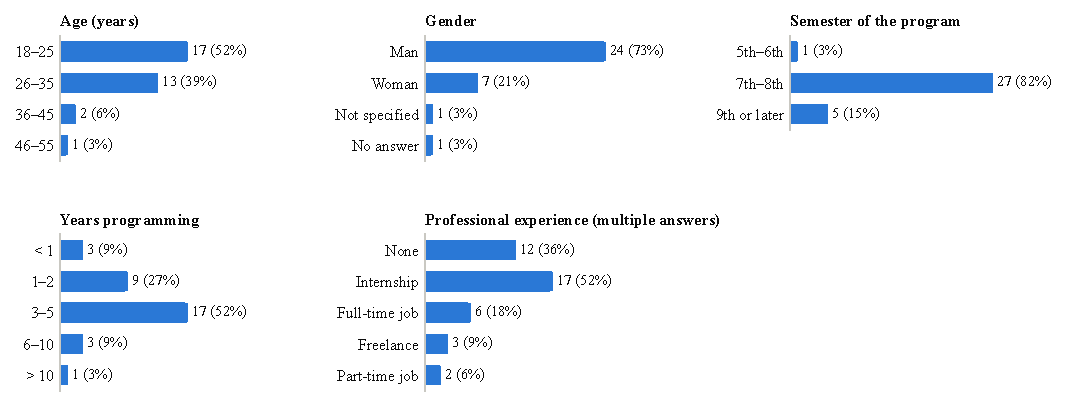
\includegraphics[width=\textwidth]{figures/participants.pdf}
\caption{Demographics and experience of the 33 respondents. Gender was an open question, coded by us. Professional experience allowed several answers; the one respondent who selected both ``none'' and an internship was counted as having an internship.}
\label{fig:participants}
\end{figure*}

\section{Results}

\subsection{RQ1: What do students build?}

The 18 applications cover a wide range of domains: booking and scheduling for sports courts, beauty salons, and medical clinics (Reservei, Estilo Marcado, MarcaConsulta); management systems for barbershops, restaurants, hospitals, internal service requests, and election operations (Trim, Mesa Clara, HealthOS, ServiceFlow, Election Ops); consumer applications for learning, game reviews, personal finance, food delivery, movies, and music (EduQuest, GameLog, Finanças, DeliveryFast, Filme Certo, Media Play); two games (CircuitCrash, Umbra Trail); a reputation service for security indicators (KapiTrace); and a tool that turns court case documents into auction notices (Leilões Judiciais).

Under the official count, the applications add up to 780,614 lines of code, with a median of 11,115 lines per project (min: 753, max: 201,848). Only three projects reached the required 100,000 lines: Trim (201,848), Umbra Trail (196,302), and DeliveryFast (137,733). Together, they account for 69\% of all the code delivered; however, as we discuss in Section~\ref{sec:gaming}, two of them reached the target mostly with generated filler. The 18 repositories have 1,051 commits, 795 (76\%) of them attributed to an agent. Claude Code was the most used agent (10 projects), followed by Codex (5), Antigravity or Gemini (5), and GitHub Copilot (3); seven teams used more than one tool, and Election Ops used five.

\subsection{RQ2: Do students follow the rules of the assignment?}

Table~\ref{tab:adherence} summarizes the adherence of the 18 projects to the methodology. Seventeen projects listed a public URL, and 17 had a \texttt{SPEC/} folder, almost always following the dated naming convention; Media Play kept four undated specifications in the layout of OpenSpec instead. Writing the specification before the code was followed only in part: among the 15 projects in which we could compute it, between 53\% and 90\% of the \texttt{Spec:}-tagged commits point to a specification added in an earlier commit. Recording sessions was the most neglected rule: three projects recorded no session at all, and four recorded a single one. The median share of commits with both \texttt{Agent:} and \texttt{Spec:} trailers is 69\%, but three projects have no commit with both. Two projects have a single human commit author, and in Mesa Clara every commit was authored by Codex. Four projects did not report the \texttt{cloc} output in the \texttt{README.md} (KapiTrace, Media Play, HealthOS, and Filme Certo), and in two projects we found strings matching API key patterns in the session exports.

\subsection{RQ3: How do students specify software for AI coding agents?}

Table~\ref{tab:specs} summarizes the 277 specifications found in the 18 repositories. Together, they add up to 261,353 words, with a median of 544 words per specification, but size varies by two orders of magnitude across projects: the median specification has 166 words in DeliveryFast, which delivered 138 thousand lines of code from three specifications, and 3,520 words in EduQuest.

\emph{RQ3.1: Who writes the specification?} The agent, in most cases. Of the 277 specifications, 191 (69\%) were added by commits attributed to an agent, only 3 (1\%) by commits explicitly declared as handwritten (\texttt{Agent: none}), and 83 (30\%) by commits that do not declare their origin. Undeclared does not mean handwritten: the four specifications of Media Play, for instance, were committed without any trailer, but the prompts recorded by the team show that they were generated by the agent from a one-paragraph description. In six projects (Trim, Finanças, Mesa Clara, CircuitCrash, Filme Certo, and MarcaConsulta), every specification was committed by an agent. Specifications committed by an agent are also the most complete: 77\% of them have acceptance criteria, against 64\% of the undeclared ones, and they are longer (median of 677 against 197 words) and less often left without any implementing commit (12\% against 69\%). This does not mean that students did not think about what to build: the prompts that produced these specifications may encode their decisions, which we plan to examine in the session logs. It does mean, however, that the artifact SDD assigns to the human was, in most projects, also written by the agent. This is not necessarily a deviation from how SDD is promoted: in GitHub Spec Kit, the coding agent drafts the specification from a high-level description, and the developer reviews it~\cite{delimarsky2025speckit}. Whether reviewing a specification gives students the same sense of ownership as writing it is one of the questions our survey addresses.

\emph{RQ3.2: Do specifications follow the required structure?} Mostly. 91\% of the specifications state what is built and why, 86\% state what is out of scope, and 74\% list acceptance criteria, with 2,196 criteria in total. The exceptions are concentrated: HealthOS describes data models, business rules, and routes, but only one of its 23 specifications has acceptance criteria; Leilões Judiciais writes long technical documents organized by layer (stack, layout, pages, tests) rather than by feature; and 13 of the 17 specifications of KapiTrace are placeholders, with the title and the sentence ``Details will be added here'', committed on the first day and never filled in.

\emph{RQ3.3: Do specifications govern the code?} Partially. 71\% of the specifications are referenced by at least one commit, and only two were referenced by commits made before they existed. However, 25\% of the specifications were added in the same commit as the code they describe, which is the case for all specifications of ServiceFlow, Leilões Judiciais, and Media Play and most of those of KapiTrace and HealthOS. Only 12\% of the specifications were edited after their implementation started, and only one explicitly replaces an earlier one, which suggests that specifications were written once, before or along with a part of the system, and rarely revisited as the system evolved. Finally, only 39\% of the lines added to the repositories come from commits that point to an existing specification. Projects that followed the trailer convention consistently, such as MarcaConsulta, DeliveryFast, Filme Certo, GameLog, and Finanças, trace more than 90\% of their lines to a specification, whereas Trim, with 63 commits marked \texttt{Spec: none}, traces only 2\%, and Umbra Trail, whose commits rarely carry a \texttt{Spec:} trailer, traces none.

\subsection{RQ4: How much ownership do students perceive?}

Section~\ref{sec:participants} describes the respondents, and Table~\ref{tab:survey} shows the distribution of their answers to all statements.

\emph{Ownership of the code is divided.} Ownership of the code has a mean of 3.29 (SD 1.14), and the answers spread over the whole scale. Only 27\% of the students agree that the code is truly theirs, and 48\% disagree. Yet 52\% agree that it reflects their own ideas, 52\% that they chose the main decisions it embodies, and 52\% would put the project in their portfolio. Five students agree that the code reflects their ideas while disagreeing that it is theirs, and four would put in their portfolio a project they do not feel is theirs, a pattern reminiscent of the AI ghostwriter effect~\cite{draxler2024}.

\emph{The ideas are mine; the code is the agent's.} The percentages make this split explicit. Students attribute to themselves a median of 50\% of the ideas of the project (Q1: 30\%, Q3: 80\%), but only 20\% of the final code (Q1: 5\%, Q3: 30\%), a significant difference (Wilcoxon signed-rank test, $p < 0.001$). 14 students (42\%) attribute at most 10\% of the code to themselves, and 5 attribute none. Students also read little of what the agent wrote: the median share of the generated code read before committing is 30\%, and 15 students (45\%) read at most a fifth of it. The median time dedicated to the assignment was 8 hours (Q1: 5, Q3: 14).

\emph{Owning the specification.} Ownership of the specification and the application has a mean of 3.27. Only 33\% of the students agree that the specification is truly theirs, which is consistent with the agent having committed most specifications (RQ3). About half agree that the specification describes the system they wanted (48\%) and that they noticed when the agent deviated from it (48\%).

\emph{Responsibility without knowledge.} Knowledge of the code is the lowest construct, with a mean of 2.71. Most students could not explain any part of the code to a colleague (58\% disagree), do not know where each feature is implemented (61\%), and could not modify the code without the agent (55\%). Still, 52\% feel responsible for its defects; of the 17 students who do, six could not modify the code without the agent.

\emph{What students say.} Thirty students answered at least one open question. The most frequent theme, in 12 answers, is a division of labor in which the ideas, the design, and the decisions belong to the student and the code belongs to the agent: ``I was the engineer of the construction, and the AI was the bricklayer; I designed and supervised. I cannot say it is totally and truly mine.'' Some students extend authorship to whoever had the idea (``even if it executes the code, authorship belongs to whoever had the idea and formulated it''), while others tie it to writing the code (``I would only truly feel that the code was mine if I wrote it 100\%''). Nine answers attribute the loss of control or of review to the pressure of the size target and the deadline: ``due to the stress of the 100 thousand lines and little time, I did not dedicate much time to reviewing the code generated by the agent, [\ldots] the project was slipping out of my control.'' Seven describe accepting code without reading it, validating only the interface, the tests, or a playtest: ``if it was working, I simply accepted it, without analyzing the code itself. [\ldots] As much as I feel I built the project, I know I do not really master the code.'' Five report the agent drifting from what they asked, sometimes unnoticed: ``the tests kept passing and the features seemed to be progressing, but [\ldots] there were still requirements of the specification that had not been implemented.'' Four describe strategies to stay in control, such as approving every commit, using a plugin that makes the agent plan and ask before deciding, writing part of the code by hand, or following SDD, which ``helped me have more authority over the project.'' Finally, two students raised the cost of agent subscriptions and token limits, which one of them considered unfair for students of a public university.

\subsection{RQ5: How does ownership relate to the footprint of the agent?}

Table~\ref{tab:corr} shows the Spearman correlations between the three ownership constructs and the other variables. Ownership is associated with what students report about their own involvement: the share of the code they attribute to themselves, the share of the generated code they read, and, to a lesser extent, the share of the ideas. It is also associated with their self-efficacy in programming and with AI tools, and with their acceptance of agents. In contrast, none of the measures mined from the repositories correlates with any ownership construct: neither the share of commits attributed to an agent, nor the share of specifications written by the agent, nor the number of recorded sessions, nor the share of lines traced to a specification, nor the share of commits authored by the respondent.

One reason may be that these measures describe the team, not the student: both members of a pair receive the same value, and almost every team delegated most of the code. Within teams, the picture changes. In the 14 pairs in which both members answered and their shares of commits differ, the member with more commits reported higher ownership of the code in 10 pairs (median of 3.64 against 2.71; Wilcoxon signed-rank test, $p = 0.046$), but not higher knowledge of the code ($p = 0.37$). Driving the agent, it seems, makes students feel the code is more theirs, without making them know it better.

\subsection{RQ6: How do students game the requirements, and what role do AI agents play?}
\label{sec:gaming}

Table~\ref{tab:gaming} summarizes what we found. The three projects that reached 100,000 lines are exactly the three in which we found generated code that the application never uses, and one of them also rewrote its history. We found no comparable pattern in the other 15 projects.

\emph{DeliveryFast: stub functions generated to reach the target.} A Python script, \texttt{gerador.py} (``generator''), writes a constant array with 24,999 entries of the form \texttt{\{ id: 4141, item: 'Produto ID 4141', price: 6211.50, active: true \}} (``Product ID 4141'') and seven component files, each with 3,999 functions of the form \texttt{renderModule\_cart\_400()}, which print a message and return a fixed HTML string. The script ends by printing ``Voluminous code generated successfully!''. These lines amount to 136,971 of the 137,705 non-blank lines of JavaScript in the project (99.5\%), and none of the generated functions or the array is imported by the application, whose actual code fits in fewer than a thousand lines. The script and its output were added in three commits within twelve minutes on October 1, two days after the assignment was released, all declaring \texttt{Agent: gemini + manual}; the second one is titled ``generates volumetric code to reach the cloc target''. The recorded session shows the exchange that produced it. The student asked: ``I need 100k lines of code. What do I have to do?''; the agent answered that ``since writing this volume by hand would be infeasible, one possibility is to use automated generation'' and proposed a first version of the script. When the student asked ``and now, how do I create the 100k lines?'', the agent scaled it up, from 1,500 to 4,000 functions per file and from 2,500 to 25,000 entries in the array.

\emph{Trim: tests that test nothing.} A script, \texttt{tests/generate\_tests.py}, writes thirteen test files, one per module of the backend, each with 1,000 test functions such as \texttt{test\_walkin\_scenario\_179}. Each test copies a dictionary defined in a fixture, adds a key, and asserts properties of the copy, such as \texttt{assert 179 <= 1000}; none of them imports any code of the application, although each file describes itself as an ``exhaustive test suite [\ldots] covering schemas, models, boundary conditions, validation, negative tests, performance considerations, and edge cases''. The 13,000 tests account for 195,147 of the 201,848 lines of the project (97\%); without them, the project has 6,701 lines. They were added in a single commit on September 30, the day after the assignment was released, declaring \texttt{Agent: antigravity/gemini-3.1-pro} and \texttt{Spec: none}, whose message reads: ``total coverage of scenarios and edge cases through dynamic fixtures; absurd increase in the metrics, reaching 200 thousand lines in the project; update of the cloc report in the README demonstrating that the 100k target was exceeded''. The team recorded no session, so we cannot tell who proposed the generator.

\emph{Umbra Trail: generated content and a rewritten history.} The third project combines two forms of gaming. First, a script writes 920 content files under \texttt{src/content}, cloned from a few templates and named, for example, \texttt{ShrineProfilePack1.ts} to \texttt{ShrineProfilePack150.ts}. Each holds six entries such as ``Auto-generated shrineprofile entry number 4141 for the content pack system'', and the files differ from each other only in numbers, identifiers, and labels such as \texttt{'even'} and \texttt{'odd'}. They add up to 57,040 lines (29\% of the count), and no file of the game imports them. In addition, the eight generator scripts add 10,884 lines to the count, mostly source code embedded as string literals that the scripts also write to \texttt{src/} (90\% to 96\% of the lines of the three largest scripts appear verbatim in \texttt{src/}), so that this code is counted twice. Without both, the project has about 128 thousand lines. The commit that added the content files was originally titled ``generated content packs (\textasciitilde104k loc)''. A day earlier, a subagent of the same tool had warned the student that creating files from \texttt{Monstro001.ts} to \texttt{Monstro999.ts} (``Monster'') ``only to reach 100 thousand lines would be artificial inflation to deceive the academic metric''.

Second, the team rewrote its history to insert specifications that did not exist. In the recorded session, on October 6, the student asked the agent: ``I need these specifications to be created from the first day of commit in the repository; it cannot be from today.'' GitHub's activity record shows what followed: at 16:23:39 that day, a member of the team created a branch named \texttt{main-antes-specs-20261006} (``main before specs''), pointing to the head of \texttt{main}; five seconds later, they force-pushed \texttt{main} to a new history; one minute later, they deleted the branch; and half an hour later, they force-pushed again. The original history, which GitHub still serves, has 39 commits and no specification at all; the delivered one has 75 commits, 22 of which add specifications. The first three commits of the delivered history are specifications dated September 29, September 30, and October 1, all at exactly 18:00:00, although the repository was created only on October 1 at 21:48, and its first commit dates from October 2. Thirteen of the 22 specification commits have timestamps with seconds equal to zero, spaced by exact intervals (e.g., 17:30:00, 17:30:20, 17:30:40), whereas in the other projects at most one specification commit per project has zero seconds, as expected by chance. The rewrite also changed the commits of the original history: their messages were translated into Portuguese, the mention of ``\textasciitilde104k loc'' disappeared, and \texttt{Agent:} trailers, absent from the original history, appeared in four commits. Consequently, the measures of specification-first development and traceability we report for this project (Tables~\ref{tab:adherence} and~\ref{tab:specs}) describe a fabricated history; in the original one, no code was preceded by a specification.

\emph{Intent, short of gaming.} In two other projects, prompts asked the agent to write code ``in more lines'' (Reservei) or to add ``rich business methods'' in order ``to reach the 100k lines'' (HealthOS), but we found no templated or unused code in them. In KapiTrace, the agent claimed in a session that the project exceeded 100,000 lines by counting its dependencies, as one of its students also reported in the survey, but the team did not report this count in its \texttt{README.md}. Conversely, the prompts of Election Ops and ServiceFlow explicitly instructed the agent not to inflate the count: ``the target of 100,000 lines must be a consequence of the functional growth of the platform, and not of artificial code''.

\emph{The role of AI agents.} The incentive to game the target was the students', and so were the decisions to commit the filler and to rewrite the history; the agents' role varied, and our evidence about it is uneven. In DeliveryFast, the only case in which the session that produced the filler was recorded, the agent did not merely execute a request: asked how to reach the target, it proposed to generate code and wrote the generator, and when asked again, it scaled the generator up. It did not point out that the generated code would not be used by the application, nor that it would defeat the purpose of the requirement. In Trim, the commit declares that the tests were produced by Antigravity, but the team recorded no session, so we cannot tell whether the student asked for filler or the agent suggested it. In Umbra Trail, the agents played opposite roles at different moments. A subagent warned the student that generating numbered files to reach the target would be ``artificial inflation to deceive the academic metric''; a day later, the content files were generated and committed, with a message announcing their size. When the student asked the agent to create specifications ``from the first day of commit'', the history was rewritten on the same afternoon; the force pushes came from a student's account, and the session does not show whether the agent or the student ran the rewrite. In sum, agents made gaming cheap, and in the one case with a recorded session they proposed it, but they did not refuse it, and the one warning we found was ignored. Agents did not create the incentive to game the target; they lowered its cost to a prompt.

\begin{table*}[t]
\centering
\caption{Requirement gaming found in the repositories. ``Lines'' and ``Share'' refer to the official \texttt{cloc} count of the project. No comparable pattern was found in the other 15 projects.}
\label{tab:gaming}
\footnotesize
\renewcommand{\arraystretch}{1.15}
\setlength{\tabcolsep}{4pt}
\begin{tabularx}{\textwidth}{@{}l >{\raggedright\arraybackslash}X r r >{\raggedright\arraybackslash}p{4.6cm} l@{}}
\toprule
\textbf{Project} & \textbf{Mechanism} & \textbf{Lines} & \textbf{Share} & \textbf{Evidence in the record} & \textbf{Agent} \\
\midrule
DeliveryFast & Script generates a 24,999-entry constant array and 27,993 stub functions; none is imported & 136,971 & 99.5\% & Commit ``generates volumetric code to reach the cloc target''; session in which the agent proposes the script & Gemini \\
Trim & Script generates 13,000 tests that import no application code & 195,147 & 97\% & Commit ``absurd increase in the metrics, reaching 200 thousand lines'' & Antigravity \\
Umbra Trail & Script generates 920 cloned content files; none is imported & 57,040 & 29\% & Original commit ``generated content packs (\textasciitilde104k loc)''; earlier warning by a subagent & Codex \\
Umbra Trail & Generator scripts embed source code also written to \texttt{src/} & 10,884 & 6\% & 90--96\% of the lines of the largest scripts appear verbatim in \texttt{src/} & Codex \\
Umbra Trail & History rewritten to insert 22 specifications, three of them dated before the repository existed & -- & -- & Prompt asking to backdate specifications; backup branch \texttt{main-antes-specs-20261006}; two force pushes; synthetic timestamps & Codex \\
\bottomrule
\end{tabularx}
\end{table*}

\begin{table}[t]
\centering
\caption{Spearman correlations between perceived ownership and self-reported and mined variables ($n = 33$). $^{*}p < 0.05$; $^{**}p < 0.01$; no correction for multiple comparisons.}
\label{tab:corr}
\footnotesize
\setlength{\tabcolsep}{3pt}
\begin{tabular}{@{}l r r r@{}}
\toprule
& \textbf{Own.} & \textbf{Own.} & \textbf{Know-} \\
& \textbf{code} & \textbf{spec/app} & \textbf{ledge} \\
\midrule
\% of ideas attributed to self & $+$0.37$^{*}$ & $+$0.36$^{*}$ & $+$0.22 \\
\% of code attributed to self & $+$0.44$^{*}$ & $+$0.21 & $+$0.49$^{**}$ \\
\% of agent code read & $+$0.43$^{*}$ & $+$0.36$^{*}$ & $+$0.35$^{*}$ \\
Hours dedicated & $+$0.28 & $+$0.23 & $+$0.25 \\
Self-efficacy in programming & $+$0.57$^{**}$ & $+$0.38$^{*}$ & $+$0.60$^{**}$ \\
Self-efficacy with AI tools & $+$0.45$^{**}$ & $+$0.39$^{*}$ & $+$0.48$^{**}$ \\
Acceptance of AI coding agents & $+$0.50$^{**}$ & $+$0.44$^{*}$ & $+$0.35$^{*}$ \\
\midrule
Own share of the team's commits & $+$0.12 & $+$0.17 & $+$0.11 \\
Team: commits by agent & $-$0.18 & $-$0.03 & $-$0.04 \\
Team: specifications by agent & $-$0.14 & $-$0.13 & $-$0.14 \\
Team: recorded sessions & $+$0.10 & $-$0.12 & $+$0.11 \\
Team: lines traced to a specification & $-$0.06 & $+$0.04 & $+$0.05 \\
\bottomrule
\end{tabular}
\end{table}

\begin{table*}[t]
\centering
\caption{Specifications per project. ``Median words'' is the median size of a specification. ``By agent'' is the share of specifications added by a commit attributed to an agent. ``Why'', ``AC'', and ``OOS'' are the shares of specifications with a section on what is built and why, with at least one acceptance criterion, and with a section on what is out of scope. ``Criteria'' counts acceptance criteria. ``Referenced'' is the share of specifications pointed to by at least one commit; ``With code'', the share added in the same commit as code; and ``Revised'', the share edited after their first implementing commit. ``Traced lines'' is the share of added lines that come from commits pointing to an existing specification.}
\label{tab:specs}
\footnotesize
\renewcommand{\arraystretch}{1.15}
\setlength{\tabcolsep}{3pt}
\begin{tabular*}{\textwidth}{@{\extracolsep{\fill}}r l r r r r r r r r r r r@{}}
\toprule
& & & & \multicolumn{1}{c}{\textbf{Authorship}} & \multicolumn{4}{c}{\textbf{Structure}} & \multicolumn{4}{c}{\textbf{Traceability}} \\
\cmidrule(lr){5-5} \cmidrule(lr){6-9} \cmidrule(l){10-13}
\textbf{ID} & \textbf{Project} & \textbf{Specs} & \textbf{Med.\ words} & \textbf{By agent} & \textbf{Why} & \textbf{AC} & \textbf{OOS} & \textbf{Criteria} & \textbf{Referenced} & \textbf{With code} & \textbf{Revised} & \textbf{Traced lines} \\
\midrule
1  & Reservei          & 15 & 328   & 87\%  & 87\%  & 40\%  & 40\%  & 53  & 93\%  & 13\%  & 13\% & 91\%  \\
2  & EduQuest          & 13 & 3,520 & 85\%  & 85\%  & 46\%  & 100\% & 88  & 92\%  & 31\%  & 46\% & 57\%  \\
3  & Trim              & 14 & 720   & 100\% & 100\% & 100\% & 100\% & 84  & 100\% & 7\%   & 0\%  & 2\%   \\
4  & KapiTrace         & 17 & 8$^{*}$ & 24\% & 12\% & 6\%   & 0\%   & 5   & 24\%  & 76\%  & 12\% & 24\%  \\
5  & GameLog           & 18 & 228   & 44\%  & 100\% & 100\% & 100\% & 168 & 100\% & 0\%   & 17\% & 96\%  \\
6  & Estilo Marcado    & 25 & 1,371 & 92\%  & 100\% & 92\%  & 100\% & 188 & 100\% & 4\%   & 12\% & 87\%  \\
7  & ServiceFlow       & 2  & 2,792 & 0\%   & 100\% & 100\% & 100\% & 31  & 100\% & 100\% & 50\% & 87\%  \\
8  & Media Play$^{\S}$  & 4  & 231   & 0\%   & 100\% & 100\% & 0\%   & 15  & 0\%   & 100\% & 0\%  & 0\%   \\
9  & Finanças          & 52 & 525   & 100\% & 100\% & 100\% & 100\% & 613 & 100\% & 13\%  & 8\%  & 92\%  \\
10 & HealthOS          & 23 & 741   & 65\%  & 100\% & 4\%   & 100\% & 7   & 35\%  & 65\%  & 4\%  & 0\%   \\
11 & DeliveryFast      & 3  & 166   & 67\%  & 100\% & 100\% & 100\% & 17  & 100\% & 0\%   & 0\%  & 100\% \\
12 & Mesa Clara        & 2  & 353   & 100\% & 100\% & 100\% & 50\%  & 15  & 100\% & 50\%  & 0\%  & 100\% \\
13 & Leilões Judiciais & 6  & 1,323 & 0\%   & 17\%  & 0\%   & 17\%  & 0   & 0\%   & 100\% & 0\%  & 0\%   \\
14 & Election Ops      & 29 & 1,164 & 52\%  & 97\%  & 79\%  & 90\%  & 319 & 62\%  & 34\%  & 3\%  & 71\%  \\
15 & CircuitCrash      & 5  & 507   & 100\% & 100\% & 20\%  & 100\% & 11  & 60\%  & 40\%  & 40\% & 28\%  \\
16 & Filme Certo       & 14 & 1,293 & 100\% & 100\% & 100\% & 100\% & 260 & 100\% & 7\%   & 50\% & 100\% \\
17 & Umbra Trail$^{\P}$ & 23 & 172   & 4\%   & 96\%  & 96\%  & 96\%  & 218 & 4\%   & 0\%   & 4\%  & 0\%   \\
18 & MarcaConsulta     & 12 & 197   & 100\% & 100\% & 100\% & 100\% & 104 & 58\%  & 0\%   & 0\%  & 99\%  \\
\midrule
   & \textbf{Total}    & \textbf{277} & \textbf{544} & \textbf{69\%} & \textbf{91\%} & \textbf{74\%} & \textbf{86\%} & \textbf{2,196} & \textbf{71\%} & \textbf{25\%} & \textbf{12\%} & \textbf{39\%} \\
\bottomrule
\multicolumn{13}{@{}p{\textwidth}@{}}{\scriptsize $^{*}$13 of the 17 specifications are placeholders with eight words. $^{\S}$Specifications in the layout of OpenSpec; acceptance criteria are \emph{WHEN}/\emph{THEN} scenarios. $^{\P}$Computed on a rewritten history; the original history has no specifications (Section~\ref{sec:gaming}).}
\end{tabular*}
\end{table*}

\begin{table*}[t]
\centering
\caption{Projects and their adherence to the methodology. ``Agents'' lists the tools declared in commit trailers and in the \texttt{README.md}, and ``Stack'' the main language and frameworks. ``Specs'' shows dated files over all specification files. ``Spec first'' is the share of \texttt{Spec:}-tagged commits whose specification was added in an earlier commit. ``Trailers'' is the share of commits with both \texttt{Agent:} and \texttt{Spec:}. ``Authors'' counts distinct human commit e-mails. ``SLOC'' uses the official \texttt{cloc} command; projects that reached 100,000 lines are highlighted in green. Other cells that fail a requirement are marked in bold.}
\label{tab:adherence}
\footnotesize
\renewcommand{\arraystretch}{1.15}
\setlength{\tabcolsep}{3pt}
\newcommand{\yes}{\checkmark}
\newcommand{\no}{\textbf{$\times$}}
\begin{tabularx}{\textwidth}{@{}r l >{\raggedright\arraybackslash}p{2.9cm} >{\raggedright\arraybackslash}X c r r r r r r c@{}}
\toprule
\textbf{ID} & \textbf{Project} & \textbf{Agents} & \textbf{Stack} & \textbf{URL} & \textbf{Specs} & \textbf{Spec first} & \textbf{Sessions} & \textbf{Trailers} & \textbf{Authors} & \textbf{SLOC} & \textbf{No secrets} \\
\midrule
1 & Reservei & Antigravity, Claude Code & TypeScript; Next.js, Supabase & \yes & 15/15 & 56\% & 14 & 49\% & 3 & 26,386 & \yes \\
2 & EduQuest & OpenCode, Claude Code & TypeScript; React, Express, Prisma & \yes & 13/13 & 58\% & 1 & 32\% & 2 & 12,580 & \yes \\
3 & Trim & Antigravity & Python; FastAPI, React & \yes & 14/14 & 53\% & \textbf{0} & 100\% & \textbf{1} & \cellcolor{green!25}201,848 & \yes \\
4 & KapiTrace & Codex, Antigravity & TypeScript; Next.js, Express, Prisma & \yes & 17/17 & 78\% & 24 & 64\% & 4 & 4,884 & \yes \\
5 & GameLog & Claude Code, Copilot & Python; Flask & \yes & 18/18 & 87\% & 4 & 82\% & 3 & 4,084 & \yes \\
6 & Estilo Marcado & Codex, DeepSeek & Java; Spring Boot, Angular & \yes & 25/25 & 72\% & 27 & 97\% & 2 & 20,516 & \no$^{\ddagger}$ \\
7 & ServiceFlow & Copilot & TypeScript; Next.js, Prisma & \yes & 2/2 & 88\% & 17 & 83\% & 2 & 9,281 & \yes \\
8 & Media Play & Antigravity & Python; Streamlit & \yes & \textbf{0/4}$^{\S}$ & -- & \textbf{0} & \textbf{0\%} & 2 & 1,262 & \yes \\
9 & Finanças & Claude Code & TypeScript; React (browser only) & \yes & 52/52 & 62\% & 51 & 66\% & 4 & 35,597 & \yes \\
10 & HealthOS & Claude Code & Python; FastAPI & \yes & 23/23 & --$^{*}$ & 1 & \textbf{0\%} & 3 & 20,850 & \yes \\
11 & DeliveryFast & ChatGPT, Gemini & JavaScript; HTML, Tailwind & \yes & 3/3 & 84\% & 1 & 92\% & 3 & \cellcolor{green!25}137,733 & \yes \\
12 & Mesa Clara & Codex & TypeScript; NestJS, Next.js, Prisma & \yes & 2/2 & 78\% & 1 & 90\% & \textbf{0}$^{\dagger}$ & 753 & \yes \\
13 & Leilões Judiciais & Claude Code & Python; FastAPI, React & \yes & 4/6 & -- & \textbf{0} & \textbf{0\%} & 2 & 9,650 & \yes \\
14 & Election Ops & Codex, Claude Code, DeepSeek, Copilot, ChatGPT & TypeScript; NestJS, React, Prisma & \no & 28/29 & 83\% & 18 & 65\% & 2 & 79,741 & \yes \\
15 & CircuitCrash & Claude Code & Python; Starlette & \yes & 5/5 & 81\% & 7 & 72\% & 3 & 3,902 & \yes \\
16 & Filme Certo & Claude Code & TypeScript; Next.js, Supabase & \yes & 14/14 & 60\% & 4 & 97\% & \textbf{1} & 9,442 & \yes \\
17 & Umbra Trail$^{\P}$ & Codex & TypeScript; Phaser & \yes & 22/23 & 75\% & 20 & \textbf{5\%} & 3 & \cellcolor{green!25}196,302 & \no$^{\ddagger}$ \\
18 & MarcaConsulta & Claude Code & Python; FastAPI, React & \yes & 12/12 & 90\% & 2 & 91\% & 2 & 5,803 & \yes \\
\bottomrule
\multicolumn{12}{@{}p{\textwidth}@{}}{\scriptsize $^{*}$\texttt{Spec:} trailers name the part of the system instead of a file path. $^{\dagger}$All commits are authored by \texttt{Codex <codex@local>}. $^{\ddagger}$API key patterns found in session exports; not manually confirmed. $^{\S}$Undated specifications in the layout of OpenSpec; prompts kept in a hand-written \texttt{prompts.md}. $^{\P}$Computed on a rewritten history; the original history has no specifications (Section~\ref{sec:gaming}).}
\end{tabularx}
\end{table*}

\section{Discussion}

\subsection{Agents Make Gaming Cheap}

Inflating a line count by hand takes effort, and its result is easy to recognize. With an agent, it takes one prompt, and the result compiles, deploys, and passes its own tests. RQ6 shows that, when a requirement can be satisfied without the engineering it is meant to elicit, some students will satisfy it that way, and agents will help them, and may even suggest how. The situation resembles \emph{specification gaming} in machine learning, in which a system satisfies the literal objective rather than the intended one. Here, however, the optimization was done by students, who had the incentive of a grade, and the agent served as a tool that made the literal objective easy to reach.

Three observations follow. First, every case was visible in the record: commit messages announce the filler, sessions show how it was produced, trailers name the agent, and GitHub's activity log exposes the rewritten history. The complete record that the assignment required, rather than the line count, is what made the gaming detectable, and it can be checked automatically. Second, the record itself can be forged: the same agent that writes code can write backdated specifications and rewrite history, so rules that live only in the repository need a source of truth outside it, such as the activity log of the hosting platform or continuous integration. Third, without the filler, only one project still reaches 100,000 lines, and the total delivered falls by about half, from 781 to roughly 380 thousand lines. The target did not measure what we wanted it to measure, and its failure is itself a finding about teaching with agents.

\subsection{Implications for Educators}

\emph{Size targets measure what the agent is good at.} The 100,000-line target was meant to make agents indispensable, and it did: no team could approach it by hand. But lines are the cheapest thing an agent produces, and the target was met unevenly: three projects produced 69\% of the code, while the median project stayed at 11,115 lines. A line count says little about the engineering behind it, and, as Section~\ref{sec:gaming} shows, it can be met with code that does nothing. Educators who want students to work at scale may set targets in terms of scope instead, such as the number of features whose acceptance criteria are demonstrably met, which also rewards the specification work the course is meant to teach.

\emph{Decide, explicitly, who writes the specification.} Our assignment required specifications to precede the code, but not that students write them, and 69\% were committed by an agent. If specifying is a learning goal, it has to be observable. A course may require a first draft of each specification committed by a student (\texttt{Agent: none}) before any agent edits it, and assess the difference between the student's draft and the final version; or, accepting that the agent drafts, assess the review instead, by asking students to record what they changed in the agent's draft and why. In both cases, an oral defense of a few acceptance criteria is a cheap check that students understand what they asked for.

\emph{Move process rules from honor to tooling.} The rules that depended on students' discipline eroded first: three teams recorded no session, a quarter of the specifications entered the repository with the code, and only 39\% of the added lines can be traced to a specification. Since agents write most commits, they can be instructed, for instance through \texttt{AGENTS.md}, to add the \texttt{Agent:} and \texttt{Spec:} trailers and to export their sessions, and a continuous integration check can reject commits without a specification or specifications added together with code. Automating the record also makes grading at this scale feasible.

\emph{Make specifications change.} Only 12\% of the specifications were revised after their implementation started, and only one replaced an earlier one. Specifications written once and never revisited teach little about how specifications work in practice. Introducing a change of requirements midway through the assignment would force students to write a new specification, decide what it replaces, and see whether the agent follows it.

\emph{Assess ownership, not only output.} A published application that opens with one click shows that the agent worked; it does not show that the students can explain, change, or defend it. In our survey, 58\% of the students could not explain any part of their code to a colleague, 55\% could not modify it without the agent, and 45\% read at most a fifth of the generated code before committing it; and the one variable under students' control that we found associated with ownership was how much of that code they read. Short oral checks, in which students locate a feature in the code or explain a decision recorded in a specification, are a practical complement to the presentation.

\subsection{Threats to Validity}

\emph{Construct validity.} Attribution to an agent relies on commit trailers, co-author lines, and bot authors; commits without them may also have been produced by an agent~\cite{kashif2026selfdeclaration}, so our counts are lower bounds. The structure of specifications was assessed through section headings and list items, which may miss content organized differently, as in HealthOS. Ownership is self-reported. \emph{Internal validity.} Students knew that the record was part of the grade, which may have shaped what they declared; the survey was not graded, but students answered it for their instructor, which may induce socially desirable answers. Our search for requirement gaming relies on heuristics that detect templated and cloned code; filler that varies more, such as verbose but distinct functions, would escape it, so the cases we report are a lower bound. Detecting rewritten histories depends on GitHub's activity record. \emph{External validity.} We study one elective course, at one university, with 18 teams, under a deliberately extreme size target; students who chose the course may be more enthusiastic about AI than their peers, and the tools evolve quickly. \emph{Conclusion validity.} With 18 teams, the relations we report in RQ5 are exploratory.

\section{Related Work}

\emph{From introductory programming to agent-built systems.} Early work on generative AI in computing education asked whether assistants help or hinder novices learning to program~\cite{kazemitabaar2023,prather2024widening}, and how instructors should respond~\cite{lau2023ban,prather2023,denny2024}. The implicit model is that the student could, in principle, write the code, and that the AI is a shortcut whose cost is lost learning. This model does not fit courses in which agents are the point. When a pair must deliver a system of tens of thousands of lines in days, the question is no longer whether students learn to write code, but what they learn to do instead (specify, review, decide) and whether they still own the result.

\emph{AI in software engineering courses.} Studies in software engineering courses have moved from perceptions to practice. Students in five courses found ChatGPT useful for coding but not for analysis and design~\cite{baresi2025students}; team projects revealed new roles and a need for transparency about who used AI for what~\cite{kharrufa2026llms,salomon2025exploration}; and Rasnayaka et al. traced AI-generated code and prompts in a course with 214 students~\cite{rasnayaka2024empirical}. In these studies, however, assistants support parts of the work, and much of the evidence on what students produced is self-reported. Vibe coding changes the picture: students rarely read the generated code~\cite{geng2026vibe} and engage little with the very practices software engineering courses exist to teach~\cite{gama2026vibes}. Recent courses respond by integrating agents deliberately, going from specification to implementation~\cite{wang2026specifications}, assessing process and reflection instead of output~\cite{fein2026aidriven}, or adopting spec-driven development~\cite{martin2026aisdlc}. These experience reports share an assumption that we put to the test: that if a course asks students to specify first, the students will be the ones specifying. None of them examines the specifications students delivered, or who wrote them.

\emph{Ownership.} Psychological ownership, the feeling that something is ``mine''~\cite{pierce2001}, matters to educators because it is tied to responsibility for one's work, and differs from the structural ownership that software engineering measures by contribution share~\cite{bird2011dont}. Research on writing shows a dissociation: people do not feel they own AI-generated text, yet claim to be its authors~\cite{draxler2024}, and more human input restores ownership only in part~\cite{joshi2025writing}. In programming, students who used ChatGPT attributed 45\% of their code to themselves, against 81\% of those who used web search~\cite{bergh2026cognition}; their sense of authorship depends on how much they refined the output~\cite{ye2026attribution}; and ownership drops as the autonomy of the AI grows~\cite{seo2026whose}. These studies rely on short tasks or vignettes, in which the work is a function or an essay. We do not know whether the dissociation holds for a system students designed, deployed, and presented, nor whether owning the specification compensates for not writing the code. Senior developers keep their agency by delegating in detail, while novices oscillate between over-reliance and avoidance~\cite{feng2026junior,huang2025dontvibe}; the specification is precisely where that detail would live.

\emph{Specification as the skill to teach.} Spec-driven tools~\cite{delimarsky2025speckit,kiro2026specs} and their academic framing~\cite{piskala2026sdd} make the specification the source of truth, and research supports making intent explicit~\cite{fakhoury2024ticoder}, to the point that validating intent has been called the central challenge of coding with agents~\cite{lahiri2026intent}. For educators, this suggests that specifying becomes the skill to teach when agents write the code. Yet the same tools let the agent draft the specification from a one-line description~\cite{delimarsky2025speckit}, which may move delegation one level up rather than remove it. Our results suggest that, for students, this risk is real.

\emph{Mining agent work.} We borrow from studies that identify agent contributions at scale through bot authors and co-author trailers~\cite{li2026aidev,zi2025agentpack}. These studies observe professionals, without access to their intentions or perceptions. Combining repository traces with a survey responds to a lesson from productivity research: how developers perceive the benefit of AI can diverge from what the evidence shows~\cite{becker2025measuring}.

\section*{Data Availability}
\label{sec:data}

\textcolor{red}{To support verification and replication, we make the following available in an artifact folder: the questionnaire in Brazilian Portuguese and its English translation; the anonymized survey responses; the list of the 18 repositories analyzed, with the commit of each one at the time of analysis; the scripts used to count lines, mine the repositories, analyze the specifications, detect requirement gaming, and analyze the survey, together with the version of \texttt{cloc} we used (1.98); and the intermediate data produced by these scripts. [Artifact URL to be added.]}

\begin{thebibliography}{00}
\bibitem{kitchenham2008} B.~A. Kitchenham and S.~L. Pfleeger, ``Personal opinion surveys,'' in \emph{Guide to Advanced Empirical Software Engineering}, F.~Shull, J.~Singer, and D.~I.~K. Sj{\o}berg, Eds. London: Springer, 2008, pp. 63--92.
\bibitem{cacioppo1982} J.~T. Cacioppo and R.~E. Petty, ``The need for cognition,'' \emph{Journal of Personality and Social Psychology}, vol.~42, no.~1, pp. 116--131, 1982.
\bibitem{davis1989} F.~D. Davis, ``Perceived usefulness, perceived ease of use, and user acceptance of information technology,'' \emph{MIS Quarterly}, vol.~13, no.~3, pp. 319--340, 1989.
\bibitem{pierce2001} J.~L. Pierce, T.~Kostova, and K.~T. Dirks, ``Toward a theory of psychological ownership in organizations,'' \emph{Academy of Management Review}, vol.~26, no.~2, pp. 298--310, 2001.
\bibitem{prather2023} J.~Prather, P.~Denny, J.~Leinonen, B.~A. Becker, I.~Albluwi, M.~Craig, H.~Keuning, N.~Kiesler, T.~Kohn, A.~Luxton-Reilly, S.~MacNeil, A.~Petersen, R.~Pettit, B.~N. Reeves, and J.~Savelka, ``The robots are here: Navigating the generative AI revolution in computing education,'' in \emph{Proc. ITiCSE Working Group Reports (ITiCSE-WGR)}. ACM, 2023, pp. 108--159.
\bibitem{denny2024} P.~Denny, J.~Prather, B.~A. Becker, J.~Finnie-Ansley, A.~Hellas, J.~Leinonen, A.~Luxton-Reilly, B.~N. Reeves, E.~A. Santos, and S.~Sarsa, ``Computing education in the era of generative AI,'' \emph{Communications of the ACM}, vol.~67, no.~2, pp. 56--67, 2024.
\bibitem{kazemitabaar2023} M.~Kazemitabaar, J.~Chow, C.~K.~T. Ma, B.~J. Ericson, D.~Weintrop, and T.~Grossman, ``Studying the effect of AI code generators on supporting novice learners in introductory programming,'' in \emph{Proc. CHI Conference on Human Factors in Computing Systems (CHI)}. ACM, 2023, pp. 1--23.
\bibitem{draxler2024} F.~Draxler, A.~Werner, F.~Lehmann, M.~Hoppe, A.~Schmidt, D.~Buschek, and R.~Welsch, ``The AI ghostwriter effect: When users do not perceive ownership of AI-generated text but self-declare as authors,'' \emph{ACM Transactions on Computer-Human Interaction}, vol.~31, no.~2, pp. 1--40, 2024.
\bibitem{lau2023ban} S.~Lau and P.~J. Guo, ``From `ban it till we understand it' to `resistance is futile': How university programming instructors plan to adapt as more students use AI code generation and explanation tools such as ChatGPT and GitHub Copilot,'' in \emph{Proc. ACM Conference on International Computing Education Research (ICER)}. ACM, 2023, pp. 106--121.
\bibitem{prather2024widening} J.~Prather, B.~N. Reeves, J.~Leinonen, S.~MacNeil, A.~S. Randrianasolo, B.~A. Becker, B.~Kimmel, J.~Wright, and B.~Briggs, ``The widening gap: The benefits and harms of generative AI for novice programmers,'' in \emph{Proc. ACM Conference on International Computing Education Research (ICER)}. ACM, 2024, pp. 469--486.
\bibitem{baresi2025students} L.~Baresi \emph{et al.}, ``Students' perception of ChatGPT in software engineering: Lessons learned from five courses,'' in \emph{Proc. IEEE/ACM 37th International Conference on Software Engineering Education and Training (CSEE\&T)}, 2025, pp. 158--169.
\bibitem{kharrufa2026llms} A.~Kharrufa, S.~Alghamdi, A.~Aziz, and C.~Bull, ``LLMs integration in software engineering team projects: Roles, impact, and a pedagogical design space for AI tools in computing education,'' \emph{ACM Transactions on Computing Education}, vol.~26, no.~2, pp. 1--27, 2026.
\bibitem{salomon2025exploration} M.~Salomon, K.~D. Chin, R.~Holmes, T.~Fritz, and G.~C. Murphy, ``An exploration of how generative AI affects workflow and collaboration in a software engineering course,'' in \emph{Proc. ACM SIGPLAN International Symposium on SPLASH-E}, 2025, pp. 42--54.
\bibitem{gama2026vibes} K.~Gama, F.~Calegario, V.~Jackson, A.~Nolte, L.~Morais, and V.~C. Garcia, ```Can you feel the vibes?': An exploration of novice programmer engagement with vibe coding,'' in \emph{Proc. IEEE/ACM 48th International Conference on Software Engineering: Software Engineering Education and Training (ICSE-SEET)}, 2026, pp. 485--496.
\bibitem{rasnayaka2024empirical} S.~Rasnayaka, G.~Wang, R.~Shariffdeen, and G.~N. Iyer, ``An empirical study on usage and perceptions of LLMs in a software engineering project,'' in \emph{Proc. 1st International Workshop on Large Language Models for Code (LLM4Code)}, 2024, pp. 111--118.
\bibitem{geng2026vibe} F.~Geng, A.~Shah, H.~Li, N.~Mulla, S.~Swanson, G.~Soosai~Raj, D.~Zingaro, and L.~Porter, ``Exploring student-AI interactions in vibe coding,'' in \emph{Proc. 28th Australasian Computing Education Conference (ACE)}, 2026, pp. 45--54.
\bibitem{wang2026specifications} Y.~Wang, M.~Beigi~Rizi, F.~Khashei, and J.~Rubin, ``From specifications to implementation in the gen-AI era: Lessons from a project-based software engineering course,'' \emph{Proceedings of the ACM on Software Engineering}, vol.~3, no.~FSE, pp. 1424--1447, 2026.
\bibitem{fein2026aidriven} B.~Fein, G.~Fraser, and S.~Herbold, ``AI-driven software development: A new course concept and assessment model for the era of large language models,'' in \emph{Proc. IEEE/ACM 48th International Conference on Software Engineering: Software Engineering Education and Training (ICSE-SEET)}, 2026, pp. 386--396.
\bibitem{martin2026aisdlc} A.~Martin and S.~Schwander, ``A lean and spec-driven AI-assisted software development lifecycle for applied AI education: The AI-SDLC approach,'' \emph{arXiv preprint arXiv:2609.24348}, 2026.
\bibitem{geng2026mapping} F.~Geng, A.~Shah, M.~Chen, P.~Denny, J.~Leinonen, B.~Griswold, G.~Soosai~Raj, and L.~Porter, ``Mapping the emerging curriculum for AI-assisted software engineering via syllabus analysis,'' \emph{arXiv preprint arXiv:2608.05898}, 2026.
\bibitem{li2026aidev} H.~Li, H.~Zhang, and A.~E. Hassan, ``AIDev: Studying AI coding agents on GitHub,'' in \emph{Proc. 23rd International Conference on Mining Software Repositories (MSR)}. ACM, 2026, pp. 1029--1033.
\bibitem{zi2025agentpack} Y.~Zi, Z.~Wu, A.~Boruch-Gruszecki, J.~Bell, and A.~Guha, ``AgentPack: A dataset of code changes, co-authored by agents and humans,'' \emph{arXiv preprint arXiv:2509.21891}, 2025.
\bibitem{becker2025measuring} J.~Becker, N.~Rush, E.~Barnes, and D.~Rein, ``Measuring the impact of early-2025 AI on experienced open-source developer productivity,'' \emph{arXiv preprint arXiv:2507.09089}, 2025.
\bibitem{kashif2026selfdeclaration} S.~M. Kashif, P.~Liang, and A.~Tahir, ``On developers' self-declaration of AI-generated code: An analysis of practices,'' \emph{ACM Transactions on Software Engineering and Methodology}, vol.~35, no.~7, pp. 1--37, 2026.
\bibitem{bird2011dont} C.~Bird, N.~Nagappan, B.~Murphy, H.~Gall, and P.~Devanbu, ``Don't touch my code! Examining the effects of ownership on software quality,'' in \emph{Proc. 19th ACM SIGSOFT Symposium and 13th European Conference on Foundations of Software Engineering (ESEC/FSE)}. ACM, 2011, pp. 4--14.
\bibitem{joshi2025writing} N.~Joshi and D.~Vogel, ``Writing with AI lowers psychological ownership, but longer prompts can help,'' in \emph{Proc. 7th ACM Conference on Conversational User Interfaces (CUI)}, 2025, pp. 1--17.
\bibitem{seo2026whose} J.~Seo, E.~Deldari, and H.~M. Mentis, ``Whose code is it? How AI autonomy reshapes ownership, responsibility, and disclosure in AI-assisted programming,'' in \emph{Proc. 31st International Conference on Intelligent User Interfaces (IUI)}. ACM, 2026, pp. 393--425.
\bibitem{bergh2026cognition} C.~Bergh, B.~Tag, A.~Vassar, and J.~Renzella, ``Your programming students' cognition with ChatGPT: Higher performance, lower retention, and reduced ownership,'' \emph{arXiv preprint arXiv:2609.21194}, 2026.
\bibitem{ye2026attribution} R.~Ye, O.~Huang, J.~He, and M.~Liut, ``Exploring emerging norms of AI attribution and disclosure in programming education,'' \emph{arXiv preprint arXiv:2602.04023}, 2026.
\bibitem{huang2025dontvibe} R.~Huang, A.~Reyna, S.~Lerner, H.~Xia, and B.~Hempel, ``Professional software developers don't vibe, they control: AI agent use for coding in 2025,'' \emph{arXiv preprint arXiv:2512.14012}, 2025.
\bibitem{feng2026junior} D.~Feng, B.~Yun, and A.~Y. Wang, ``From junior to senior: Allocating agency and navigating professional growth in agentic AI-mediated software engineering,'' in \emph{Proc. CHI Conference on Human Factors in Computing Systems (CHI)}. ACM, 2026, pp. 1--24.
\bibitem{delimarsky2025speckit} D.~Delimarsky, ``Spec-driven development with AI: Get started with a new open source toolkit,'' GitHub Blog, Sep. 2025. [Online]. Available: \url{https://github.blog/ai-and-ml/generative-ai/spec-driven-development-with-ai-get-started-with-a-new-open-source-toolkit/}
\bibitem{kiro2026specs} Kiro, ``Specs,'' Kiro Documentation. [Online]. Available: \url{https://kiro.dev/docs/specs/}. Accessed: Oct. 7, 2026.
\bibitem{piskala2026sdd} D.~B. Piskala, ``Spec-driven development: From code to contract in the age of AI coding assistants,'' \emph{arXiv preprint arXiv:2602.00180}, 2026.
\bibitem{fakhoury2024ticoder} S.~Fakhoury, A.~Naik, G.~Sakkas, S.~Chakraborty, and S.~K. Lahiri, ``LLM-based test-driven interactive code generation: User study and empirical evaluation,'' \emph{IEEE Transactions on Software Engineering}, vol.~50, no.~9, pp. 2254--2268, 2024.
\bibitem{lahiri2026intent} S.~K. Lahiri, ``Intent formalization: A grand challenge for reliable coding in the age of AI agents,'' \emph{arXiv preprint arXiv:2603.17150}, 2026.
\end{thebibliography}

\end{document}
